\documentclass[a4paper,10pt]{article}
\usepackage[utf8]{inputenc}
\usepackage[a4paper,margin=3.5cm]{geometry} %Sets the page geometry
\usepackage{url}
\usepackage{dirtytalk}
\usepackage{graphicx} % Package for \includegraphics
\usepackage{wrapfig} % Figure wrapping
\usepackage[T1]{fontenc} % Output font encoding for international characters
\setlength{\parskip}{1em} % Set space when paragraphs are used
\usepackage{amssymb}
\usepackage{amsmath}
\usepackage{tcolorbox}
\usepackage{mathtools}
\usepackage{tikz}
\usepackage{amsthm}
\usepackage{caption}
\usepackage{changepage}
\usetikzlibrary{arrows}

% Self Explanatory
\newtheorem{theorem}{Theorem}[section]
\newtheorem{definition}{Definition}[section]
\newtheorem{corollary}{Corollary}[theorem]
\newtheorem{lemma}[theorem]{Lemma}
\newtheorem{exercise}{Exercise}[section]

\theoremstyle{definition} % Set solutions to be bold
\newtheorem*{solution}{Solution}

% Other
\DeclarePairedDelimiter\floor{\lfloor}{\rfloor} %Floor function

% Remove indentation for paragraphs
\setlength{\parindent}{0pt}

\def\changemargin#1#2{\list{}{\rightmargin#2\leftmargin#1}\item[]}
\let\endchangemargin=\endlist 

% Change footnote numbering to numeric style
\renewcommand{\thefootnote}{\arabic{footnote}}


\begin{document}
    \section{Lecture 01}
    This course deals with \emph{abstract mathematical objects}, which
    are defined by the properties they satisfy.

    \textbf{Properties:} defined by propositions/statements which are either true or false. 
    Here are a few examples of propositions:
    \begin{enumerate}
        \item 7 is a prime number.
        \item All natural numbers are even.
        \item All even numbers greater than 2 can be written as the sum of 2 primes.
    \end{enumerate}

    We shall try to define the natural numbers themselves using the properties 
    they satisfy. Let's start with these 2 axioms:

    \begin{tcolorbox}[colback=blue!10!white, colframe=blue!50!black]
    \begin{enumerate}
        \item $0$ is a natural number. \footnotemark
        \item For every natural number $n$, there exists a natural number $n+1$.
    \end{enumerate}
    \end{tcolorbox}
    \footnotetext{Whether we add 0 or not to the set of natural numbers is simply a 
    matter of convention. For this course, it is convenient to add it to the set.}

    The first axiom tells us that there is a starting number (which we call 0), 
    and the second axiom tells us that for every natural number there is a \emph{next} 
    natural number.

    It might be a bit weird to use the addition symbol in our axioms when we haven't 
    even defined numbers yet. Note that this is just a notation; to make it clear
    we can write $next(n)$ instead of $n+1$ to indicate the next natural number. 
    It's best to think of $next(n)$ as a function which just spits out a new natural
    number for each input $n$.

    \textbf{Predicates: }a statement which involves variables, which can take any value
    in some domain. Think of a predicate $P(x)$ as a function which assign true or 
    false to each value x. For example, $P(x)$ could denote \emph{x is the square of
    an integer}.

    There are 3 ways to make a predicate into a proposition:
    \begin{enumerate}
        \item Substitute a constant for x, for example $P(18)$ is a proposition.
        \item $\exists x \ P(x)$: this proposition is true if there is some object
        $a$ for which $P(a)$ is true.
        \item $\forall x \ P(x)$: this proposition is true if $P(x)$ is true for all
        objects x. 
    \end{enumerate}

    Using this notation, we can precisely write our previous 2 axioms for natural numbers:
    \begin{tcolorbox}[colback=blue!10!white, colframe=blue!50!black]
    \begin{enumerate}
        \item $\exists n \ n = 0$
        \item $\forall n \ \exists m \ (m = next(n))$
    \end{enumerate}
    \end{tcolorbox}

    Let's think more about the second axiom. We need to place more restrictions on this 
    \emph{next} function to get our natural numbers. For example, if we allow $next(0) = 0$, 
    our natural numbers just becomes the set $\{0\}$, and it satisfies the axioms we have so far.
    We could also have $next(0) = 1, next(1) = 0$. So one restriction we could think of to
    avoid this is to keep $next(n) \neq 0$ for all $n$.

    \begin{figure}[ht]
    \centering
    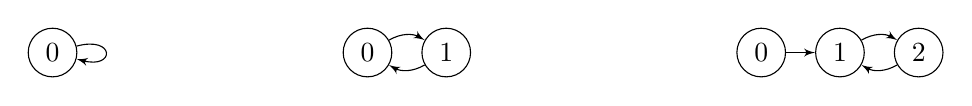
\begin{tikzpicture}
        \tikzset{vertex/.style = {shape=circle,draw,minimum size=1.5em}}
        \tikzset{edge/.style = {->,> = latex'}}
        % vertices
        \node[vertex] (a0) at (0,0) {0};
        \node[vertex] (b0) at (4,0) {0};
        \node[vertex] (b1) at (5,0) {1};
        \node[vertex] (c0) at (9,0) {0};
        \node[vertex] (c1) at (10,0) {1};
        \node[vertex] (c2) at (11,0) {2};
        %edges
        \draw[edge] (a0) to [loop right] ();
        \draw[edge] (b0) to [bend left] (b1);
        \draw[edge] (b1) to [bend left] (b0);
        \draw[edge] (c0) to (c1);
        \draw[edge] (c1) to [bend left] (c2);
        \draw[edge] (c2) to [bend left] (c1);
        
    \end{tikzpicture}

    \caption[Caption for LOF]{Valid number systems\footnotemark\ without any condition
    on \emph{next}}
    \end{figure}
    \footnotetext{It's important to keep in mind what makes one number system different
    from another is how the nodes are linked, it's not about what symbol we keep for each
    node like 0, 1, 2}

    Is this enough? Not really, as we can still think of counterexamples, like
    $next(0) = 1, next(1) = 2, next(2) = 1$. Basically we have ensured that \emph{next}
    doesn't loop back to 0. But we must ensure that it doesn't loop back at all 
    (or even to the same number). How we shall do this is to add the restriction that 
    \emph{next} should not point to a number which has already been mapped to i.e. we make
    it a one-one function. Let's now add these conditions to our axioms:

    \begin{tcolorbox}[colback=blue!10!white, colframe=blue!50!black]
        \begin{enumerate}
            \item $\exists n \ n = 0$
            \item $\forall n \ \exists m \ (m = next(n))$
            \begin{enumerate}
                \item $\forall n \ next(n) \neq 0$
                \item $\forall m \ \forall n \ next(m) = next(n) \implies m = n$
            \end{enumerate}
        \end{enumerate}
    \end{tcolorbox}

    \begin{figure}[ht]
    \centering
    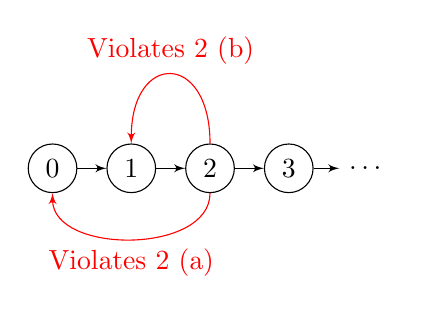
\begin{tikzpicture}
        \tikzset{vertex/.style = {shape=circle,draw,minimum size=1.5em}}
        \tikzset{edge/.style = {->,> = latex'}}
        % vertices
        \node[vertex] (0) at (0,0) {0};
        \node[vertex] (1) at (1,0) {1};
        \node[vertex] (2) at (2,0) {2};
        \node[vertex] (3) at (3,0) {3};
        \node (ellipsis) at (4,0) {\ldots};
        %edges
        \draw[edge] (0) to (1);
        \draw[edge] (1) to (2);
        \draw[edge] (2) to (3);
        \draw[edge] (3) to (ellipsis);
        \draw[red, edge] (2) to [in=90, out=90, looseness=3] node[midway, above] {Violates 2 (b)} (1);
        \draw[red, edge] (2) to [in=270, out=270, looseness=1] node[midway, below] {Violates 2 (a)} (0);
    \end{tikzpicture}
    \caption{Diagrammatic explanation of why \emph{next} always points to a new number}
    \end{figure}

    It turns out our axioms are still not complete. We have ensured that \emph{next}
    always points to a new number, but we haven't really ensured that every natural
    number can be formed by applying \emph{next} to 0 a finite number of times. 
    Here are some counterexamples:
    \begin{enumerate}
        \item $\left\{0, \frac{1}{3}, \frac{2}{3}, \dots\right\}$ where $next(n) = n+1$ 
        \item $[0, \infty)$ where $next(n) = n+1$
    \end{enumerate}
    
    By repeatedly applying \emph{next} to our growing chain, we should end up 
    with the set of all natural numbers. A neat way of stating this is to just
    keep an axiom that induction itself works i.e. if a statement is true for 
    $0, next(0), next(next(0)), \dots$ it must be true for all natural numbers.
    So here is our final set of axioms, which does lead only to our natural numbers:

    \begin{tcolorbox}[colback=blue!10!white, colframe=blue!50!black]
        \begin{enumerate}
            \item $\exists n \ n = 0$
            \item $\forall n \ \exists m \ (m = next(n))$
            \begin{enumerate}
                \item $\forall n \ next(n) \neq 0$
                \item $\forall m \ \forall n \ next(m) = next(n) \implies m = n$
            \end{enumerate}
            \item $[P(0)]  [\forall n \ \{P(n) \implies P(next(n))\}] \implies [\forall n \ P(n)]$
        \end{enumerate}
    \end{tcolorbox}

    \begin{exercise}
        Prove that $\forall n \ next(n) \neq n$. Can we have this statement instead of 
        2 (b) to define natural numbers?
    \end{exercise}
    \begin{solution}
        Proof by induction \\
        Define $P(n)$ to be $\ next(n) \neq n$. $P(0)$ is true from 2 (a). \\
        Also, $next(n) \neq n \implies next(next(n)) \neq next(n)$ as \emph{next} is one-
        one (or contrapositive of 2 (b)). This is basically $P(n) \implies P(next(n))$. \\
        From this we conclude $P(n)$ i.e. $next(n) \neq n$ for all $n$. \\
        This can't be used instead of 2 (b). Counterexample: $next(0) = 1, next(1) = 2, next(2) = 1$.
    \end{solution}

    \begin{exercise}
        Instead of keeping induction as an axiom, we could ensure that there are no other
        starting points for a chain other than 0. This might ensure that all numbers are
        part of the chain starting from 0. 

        Can we replace axiom 3 with the following: \\ 
        $\forall n \ n \neq 0 \iff \exists m \ next(m) = n$
    \end{exercise}
    \begin{solution}
        No, we have a counterexample, take the set \\ 
        $\{0, 1, 2, \dots\} \cup \{\dots, -1.5, -0.5, 0.5, 1.5, \dots\}$ where $next(n)$ is the standard $n+1$. \\
        It satisfies the new set of 3 axioms but aren't equivalent to natural numbers.
    \end{solution}

    \begin{exercise}
        Is there a more concrete way to show that from axiom 3 that all natural numbers
        can be obtained composing $next$ to 0 a finite (including 0) number of times?
    \end{exercise}
    \begin{solution}
        Let $P(n)$ denote $n$ obtained composing \emph(next) to 0 a finite (including 0) 
        number of times. $P(0)$ is obviously true. It's also clear that $P(n) \implies P(next(n))$,
        as if $n$ can be written as $next(next(\dots(next(0))\dots))$, $next(n)$ can also be written
        that way by just composing one more \emph{next} to the expression. 
        This completes our proof.

        Another way we can do this question is proof by contradiction.
        Assume there are some numbers not in the infinite chain starting from 0.
        We define our predicate to be true for values in the infinite chain starting
        from 0, and false for every other value.

        \begin{figure}[ht]
            \centering
            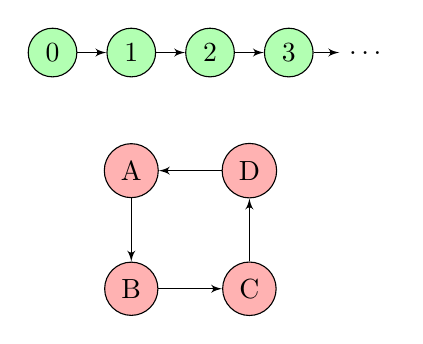
\begin{tikzpicture}
                \tikzset{vertex/.style = {shape=circle,draw,minimum size=1.5em}}
                \tikzset{edge/.style = {->,> = latex'}}
                % vertices
                \node[vertex, fill=green!30] (0) at (0,0) {0};
                \node[vertex, fill=green!30] (1) at (1,0) {1};
                \node[vertex, fill=green!30] (2) at (2,0) {2};
                \node[vertex, fill=green!30] (3) at (3,0) {3};
                \node (ellipsis) at (4,0) {\ldots};

                \node[vertex, fill=red!30] (a) at (1,-1.5) {A};
                \node[vertex, fill=red!30] (b) at (1,-3) {B};
                \node[vertex, fill=red!30] (c) at (2.5,-3) {C};
                \node[vertex, fill=red!30] (d) at (2.5,-1.5) {D};
                %edges
                \draw[edge] (0) to (1);
                \draw[edge] (1) to (2);
                \draw[edge] (2) to (3);
                \draw[edge] (3) to (ellipsis);

                \draw[edge] (a) to (b);
                \draw[edge] (b) to (c);
                \draw[edge] (c) to (d);
                \draw[edge] (d) to (a);
            \end{tikzpicture}
            \caption{Our predicate is true for green cells and false for the red cells}
            \end{figure}
    \end{solution}

    This predicate satisfies $P(0)$ is true. It also satisfies $P(n) \implies P(next(n))$,
    because if $P(n)$ is true only for the green cells, and green cells point to only green cells.
    So induction steps are done, but $P(n) \forall n$ is false. So we have a contradiction.

    \section{Lecture 02}

    To extend our definition, let's define $\leq$ operator.

    \begin{tcolorbox}[colback=blue!10!white, colframe=blue!50!black]
        \begin{enumerate}
            \item $\forall n \ \leq(0, n)$ is true
            \item $\forall n \ \leq(next(n), 0)$ is false
            \item $\forall n \  \forall m \ [\leq(next(n), next(m))\ = \ \leq(n, m)]$
        \end{enumerate}
    \end{tcolorbox}

    \begin{figure}[ht]
    \centering
    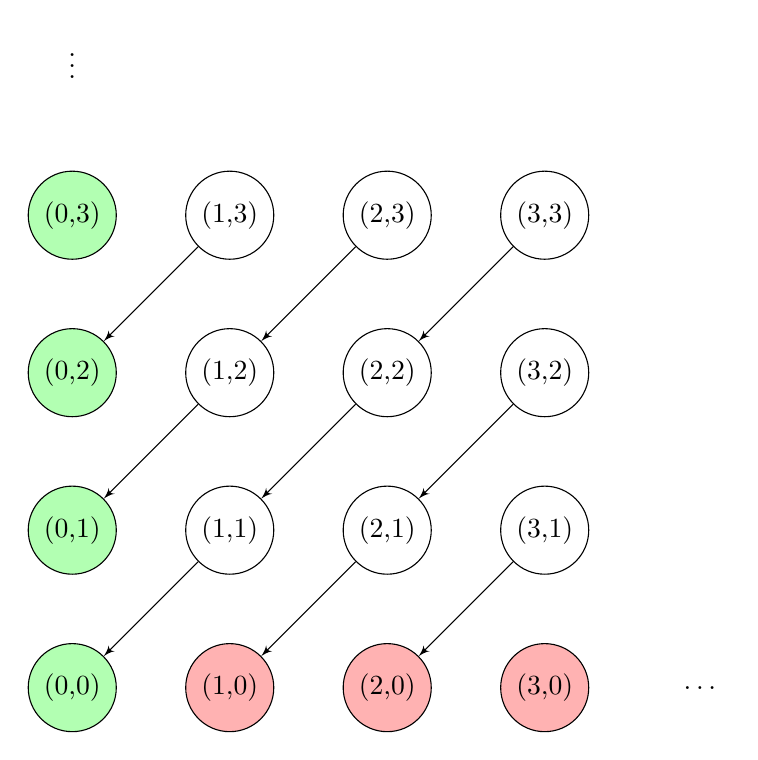
\begin{tikzpicture}
        \tikzset{vertex/.style = {shape=circle,draw,minimum size=1.5em}}
        \tikzset{edge/.style = {->,> = latex'}}

        % vertices
        \foreach \x in {0,...,3}
            \node[vertex, fill=green!30] (0-\x) at (0, 2*\x) {(0,\x)};
        \node (e1) at (0,8) {\vdots};

        \foreach \y in {1,2,3}
            \node[vertex, fill=red!30] (\y-0) at (2*\y,0) {(\y,0)};
        \node (e2) at (8,0) {\ldots};

        \foreach \x in {1,2,3}
            \foreach \y in {1,2,3}
                \node[vertex] (\x-\y) at (2*\x,2*\y) {(\x,\y)};
        

        %edges
        \draw[edge] (1-1) to (0-0);
        \draw[edge] (2-2) to (1-1);
        \draw[edge] (3-3) to (2-2);
        \draw[edge] (2-1) to (1-0);
        \draw[edge] (1-2) to (0-1);
        \draw[edge] (2-3) to (1-2);
        \draw[edge] (3-2) to (2-1);
        \draw[edge] (1-3) to (0-2);
        \draw[edge] (3-1) to (2-0);

    \end{tikzpicture}
    \captionsetup{justification=centering}  % <-- Center the caption
    \caption{Diagrammatic representation of how $\leq$ is defined \\
    $\leq$ is defined as true for green cells, false for red cells \\
    $(A) \rightarrow (B)$ denotes $(A)$ is defined by $(B)$}
    \end{figure}

    From the figure it's intuitive (hopefully) that $\leq(m,n)$ is defined for all $m$ and $n$,
    (3) kind of gives a recursive definition. 
    But how do we prove this? Since our predicate has 2 input variables, there
    is some sort of nested induction.\\
    Take $P(m)$ to be $\forall n \ \leq(m,n)$ is defined. \\
    $P(0)$ is defined from (1).\\
    Now assume $\forall n \ \leq(m,n)$ is defined (which is $P(m)$) \\
    We have to prove $\forall n \ \leq(next(m),n)$ is defined (which is $P(next(m)))$ \\
    The thing is, there's no direct way to proceed from here. It's clear that we somehow
    want to use (3) but we can't as we have $\leq(next(m),n)$ instead of $\leq(next(m),next(n))$.
    How we proceed is we take $Q(n)$ as $\leq(next(m),n)$ is defined, which is want we want to prove
    to complete the induction, and prove $Q(n)$ using induction itself!
    (Note that for the $Q(n)$ statement, $m$ is fixed!)
    $Q(0)$ is true as $\leq (next(m), 0)$ is defined as false. \\
    Now assume $Q(n)$ is true i.e. $\leq(next(m),n)$ is defined. \\
    $Q(next(n))$ is $\leq(next(m),next(n))$ which is $\leq(m,n)$ which is defined, as it is $P(m)$.
    So we proved $\forall n \ Q(n)$, which is the inner induction complete. \\
    This also completes the outer induction.

    \begin{exercise}
        Prove that $\leq(a,b) \ \land \ \leq(b,a) \implies a = b$
    \end{exercise}
    \begin{solution}
        Nested induction on $a$, $b$.\\
        Let $P(a)$ be $\forall b \ \leq(a,b) \ \land \ \leq(b,a) \implies a = b$ \\
        First we need to show that $P(0)$ is true. $\leq(0,b)$ is always true, also
        we can see that $\leq(b,0)$ is true implies $b$ is $0$ as if it's not the case,
        $b$ can be written as $next(k)$ and $\leq(next(k),0)$ is false. \\
        Now for the induction, assume $\leq(a,b) \ \land \ \leq(b,a) \implies a = b$ \quad ($\ast$)\\
        To prove: $\leq(next(a),b) \ \land \ \leq(b,next(a)) \implies next(a) = b$ \\
        Nested induction now, take the above as $P(b)$. 
        \begin{adjustwidth}{2cm}{0cm}
            $P(0)$ is a vacuous truth as $\leq(next(a),0)$ is false. \\
            Now assuming $P(b)$ we have to prove $P(next(b))$, which is \\
            $\leq(next(a),next(b)) \ \land \ \leq(next(b),next(a)) \implies next(a) = next(b)$ \\
            But this is just equivalent to ($\ast$), as LHS of the implication can be 
            simplified by the recursive definition of $\leq$ and RHS of the implication can be 
            simplified with one-oneness of \emph{next}. \\
            So inner induction is complete.
        \end{adjustwidth}
        This also completes outer induction as we have proved $\forall b \ P(b)$
    \end{solution}

    \begin{exercise}
        Prove that $\leq(a,b) \ \land \ \leq(b,c) \implies \leq(a,c)$
    \end{exercise}
    \begin{solution}
        Nested induction again\dots \\
        Let $P(a)$: $\forall b \ \forall c \ \leq(a,b) \ \land \ \leq(b,c) \ \implies \ \leq(a,c)$ \\
        $P(0)$ is true as RHS of implication is always true. \\
        Now assume $P(a)$: $\forall b \ \forall c \ \leq(a,b) \ \land \ \leq(b,c) \ \implies \ \leq(a,c)$ \quad $(\ast)$ \\
        To prove $P(next(a))$: $\forall b \ \forall c \ \leq(next(a),b) \ \land \ \leq(b,c) \ \implies \ \leq(next(a),c)$
        \begin{adjustwidth}{1cm}{0cm}
            Let $Q(b)$: $\forall c \ \leq(next(a),b) \ \land \ \leq(b,c) \ \implies \ \leq(next(a),c)$ \\
            $Q(0)$ is true as first term of LHS of implication is false. \\
            Now assuming $Q(b)$ we have to prove $Q(next(b))$, which is: \\
            $\forall c \ \leq(next(a),next(b)) \ \land \ \leq(next(b),c) \ \implies \ \leq(next(a),c)$
            \begin{adjustwidth}{1cm}{0cm}
                Let $R(c)$: $\leq(next(a),next(b)) \ \land \ \leq(next(b),c) \ \implies \ \leq(next(a),c)$ \\
                $R(0)$ is true as second term of LHS of implication is false. \\
                Now assume $R(c)$, we have to prove $R(next(c))$, which is: \\
                $\leq(next(a),next(b)) \ \land \ \leq(next(b),next(c)) \ \implies \ \leq(next(a),next(c))$ \\
                This can be reduced by the recursive definition to ($\ast$) which is assumed as true.
            \end{adjustwidth} 
        \end{adjustwidth}
        That completes all the induction layers.
    \end{solution}

    \begin{exercise}
        Prove that $\leq(a, next(b)) \ \implies \ [\leq(a,b)] \lor [a=next(b)]$ \\
        Use this to prove $[\leq(a,b)] \land [\leq(b,next(a))] \ \implies \ [b=a] \lor [b=next(a)]$
    \end{exercise}
    \begin{solution}
        Let $P(a)$: $\forall b \ \leq(a, next(b)) \ \implies \ [\leq(a,b)] \lor [a=next(b)]$ \\
        $P(0)$ is true as $\leq(0,b)$ is always true. \\
        Now assuming $P(a)$, we have to prove $P(next(a))$.
        \begin{adjustwidth}{1cm}{0cm}
            Let $Q(b)$: $\leq(next(a), next(b)) \ \implies \ [\leq(next(a),b)] \lor [next(a)=next(b)]$ \\
            $Q(0)$: $\leq(a, 1) \ \implies \ [\leq(a,0)] \lor [a=1]$ \\
            We can first simplify $\leq(a,0)$ to $a=0$ using Exercise 2.1's property. \\
            Let's take $Q(0)$ as $R(a)$ and prove that using induction.
            \newpage
            \begin{adjustwidth}{1cm}{0cm}
                $R(0)$ is true as $\leq(a,0)$ is true. \\
                Now assuming $R(a)$ we have to prove $R(next(a))$. \\
                $\leq(next(a),1) \implies \leq(a,0) \implies a=0 \implies next(a)=1$ so $R(next(a))$ is true \\
                So $R(a)$ is true for all a.
            \end{adjustwidth}
            Now assuming $Q(b)$ we have to prove $Q(next(b))$ \\
            But that can be reduced to just $P(a)$ which is assumed as true. \\
            This completes the induction.
        \end{adjustwidth}
        
        For the second part, we know : \\
        $\leq(b, next(a)) \ \implies \ [\leq(b, a)] \lor [b = next(a)]$ \\
        And if $\leq(b, a)$ since we also know $\leq(a, b)$, $b = a$.

        This exercise shows that there is no number in-between $n$ and $next(n)$ 
    \end{solution}

    We now define the addition function $add(m, n)$: 
    \begin{tcolorbox}[colback=blue!10!white, colframe=blue!50!black]
        \begin{enumerate}
            \item $add(0, m) = m$
            \item $add(next(n), m) = next(add(n, m))$
        \end{enumerate}
    \end{tcolorbox}
    It's not too hard to show this sufficiently defines addition by taking $P(n)$ as
    [$add(n, m)$ is defined] and using induction.

    \begin{exercise}
        Prove that $add(add(a,b), c) = add(a, add(b,c))$ which is the associative property
    \end{exercise}
    \begin{solution}
        We can somehow avoid nested induction for once :) \\
        Let $P(a)$ be $\forall b \ \forall c \ add(add(a,b), c) = add(a, add(b,c))$ \\
        To prove $P(0)$, $LHS = add(add(0,b), c) = add(b,c)$ and $RHS = add(0, add(b,c)) = add(b,c)$ \\
        To prove $P(next(a))$, assuming $P(a)$ is true: \\
        $LHS = add(add(next(a),b), c) = add(next(add(a,b)), c) = next(add(add(a,b), c))$ \\
        $RHS = add(next(a), add(b,c)) = next(add(a, add(b,c)))$ \\
        And from $P(a)$ these both are equal.
    \end{solution}

    \begin{exercise}
        Prove that $add(a,b) = add(b,a)$ which is the commutative property
    \end{exercise}
    \begin{solution}
        Lot of induction again :( \\
        Let $P(a)$ be $\forall b \ add(a,b) = add(b,a)$ \\
        $P(0)$ is $\forall b \ add(0,b) = b = add(b,0)$, this itself has to be done by induction on b. \\
        Now assume $P(a)$ which is $\forall b \ add(a,b) = add(b,a)$ \quad ($\ast$) \\
        Basically whenever we have $a$ in the add function we can swap stuff. \\
        To prove: $P(next(a))$ which is $\forall b \ add(next(a),b) = add(b,next(a))$ \\
        We can simplify LHS a bit: $add(next(a),b) = next(add(a,b)) = next(add(b,a))$ from ($\ast$)
        \begin{adjustwidth}{1cm}{0cm}
            Let $Q(b)$ be $add(b, next(a)) = next(add(b,a))$ \quad ($\ast\ast$) \\
            $Q(0)$ is true as we get $LHS = RHS = next(a)$ \\
            Now assume $Q(b)$, we have to prove $Q(next(b))$ \\
            LHS for this is $add(next(b), next(a)) = next(add(b, next(a)))$ \\
            RHS is $next(add(next(b,a)))$ which is $next(next(add(b,a)))$ \\
            And from ($\ast\ast$) both of these are equal
        \end{adjustwidth}
        This completes all the induction.
    \end{solution}

    \newpage
    \begin{exercise}
        Prove that $\leq(a,b) \ \implies \ \exists c$ such that $add(a,c) = b$
    \end{exercise}
    \begin{solution}
        Let $P(a)$ be the above statement for all $b$. \\
        $P(0)$ is true as $c = b$ works. \\ 
        Now assume $P(a)$ is true. \quad ($\ast$) \\
        We have to prove $P(next(a))$, take this as $Q(b)$.
        \begin{adjustwidth}{1cm}{0cm}
            $Q(0)$ is vacuously true as $\leq(next(a), 0)$ is false. \\
            Now assuming $Q(b)$ we have to prove $Q(next(b))$ \\
            $\leq(next(a), next(b)) \ \implies \ \leq(a,b)$ \\
            So from ($\ast$) we know $\exists c$ such that $add(a,c) = b$ \\
            But this also implies $add(next(a), c) = next(b)$ \\
            This proves $Q(next(b))$ which completes all the induction.
        \end{adjustwidth}
        This exerise in a way defines subtraction, $c = b-a$
    \end{solution}

    \section{Lecture 03}
    Rather than using induction, there's an equivalent way to define natural numbers called
    well-ordering principle. Here are the axioms:

    \begin{tcolorbox}[colback=blue!10!white, colframe=blue!50!black]
        \begin{enumerate}
            \item $\exists n \ n = 0$
            \item $\forall n \ \exists m \ (m = next(n))$
            \begin{enumerate}
                \item $\forall n \ next(n) \neq 0$
                \item $\forall m \ \forall n \ next(m) = next(n) \implies m = n$
                \item $\forall n \ [n = 0] \lor [\exists m \ n = next(m)]$
            \end{enumerate}
            \item $\exists \ \leq$
            \begin{enumerate}
                \item $\forall n \ \lnot \leq(next(n), n)$
                \item $\forall P \ [(\exists n \ P(n)) \ \implies \ \exists n \ (P(n) \ \land \ \forall m(P(m) \implies n \leq m))]$
            \end{enumerate}
        \end{enumerate}
    \end{tcolorbox}

    This might look like it's very complicated using predicate logic, so let's try to see
    what all this means. So the beginning is pretty much like the previous axioms, but 2(c)
    is new. It basically says every number is either 0 or is the \emph{next} of some other number.
    We'll later see how this axiom helps in proving induction itself.

    What does the third axiom say? It says there exists \textbf{some} predicate $\leq$, which 
    is not necessarily the $\leq$ we saw in Lecture 02. But anyways there's some predicate
    $\leq$ which `orders' the natural numbers. What exactly do we mean by that? 3(a) says
    \emph{next} of any number is greater than it. 3(b) says that for all predicates $P$, if
    there is at least one number for which $P$ is true, there will a `smallest' number for
    which it is true. How we write this formally is that there is some $n$ for which $P(n)$ is
    true and for every other $m$ for which it is true, $n \leq m$.

    Let's see how induction is true from these axioms. We prove induction by contradiction.
    Assume there is a predicate $P$ such that $P(0)$ is true, and $P(n) \implies P(next(n))$.
    But $\forall n \ P(n)$ is false, that is there's some $n$ for which $\lnot P(n)$ is true.
    Let the smallest $n$ that satisfies this be $n_0$ (we're using 3(b) here).
    $n_0 \neq 0$ as $P(0)$ is true. So from 2(c) there's $m$ such that $next(m) = n_0$.
    Is $P(m)$ true? If it was, $P(m) \implies P(next(m))$, which would make $P(n_0)$ true.

    So $P(m)$ is false, but haven't we just found a number smaller than $n_0$ which satisfies
    $\lnot P(n)$, which contradicts well-ordering? From 3(a) we know $\leq(n, m)$ is false\footnote
    {Without 3(a) we can't actually conclude this, remember this isn't our familiar
    $\leq$, this is just an arbitrary predicate which satisfies well-ordering}.
    So from 3(b) we can get our contradiction, but remember the predicate we are using is 
    $\lnot P$ instead of $P$. We have $n$ such that $\lnot P(n)$, so 3(b) guarantees
    there exists $n_0$ such that $\lnot P(n)$ is true, and for all other $m$ that
    satisfies $\lnot P(n)$, $\leq(n,m)$. So 3(a) and 3(b) form our contradiction.

    \begin{exercise}
        We have seen how 2(c) was used in proving induction, but maybe even without it
        maybe we get only natural numbers? Is there a number system which isn't natural numbers
        but satisfies everything except 2(c)?
    \end{exercise}

    \begin{solution}
        In fact there are.
        $\{0, 1, 2, \dots, \omega, \omega+1, \omega+2, \dots\}$ form a number system. \\
        Here $\leq$ is what you'd expect it to be, the numbers are arranged in order 
        already, and $\omega$ is greater than all the natural numbers. 
        $\leq$ satisfies all the properties it needs to, even things like 
        the transitive property. But 2(c) forbids such things are there is no $n$
        such that $next(n) = \omega$. These are actually called the ordinal numbers.
        Thing is, we get many useful number systems if we make small changes to our axioms,
        for example if we remove $next(n) \neq 0$ we get modular arithmetic.

        \begin{figure}[ht]
            \centering
            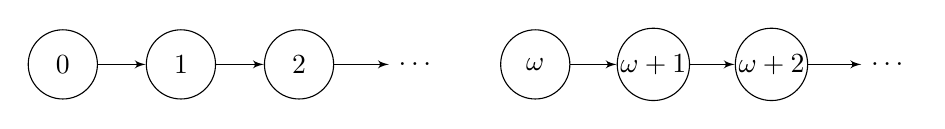
\begin{tikzpicture}
                \tikzset{vertex/.style = {shape=circle,draw,minimum size=2.5em}}
                \tikzset{edge/.style = {->,> = latex'}}
                % vertices
                \node[vertex] (0) at (0,0) {0};
                \node[vertex] (1) at (1.5,0) {1};
                \node[vertex] (2) at (3,0) {2};
                \node (e1) at (4.5,0) {\ldots};
                \node[vertex, inner sep=0.5pt] (w) at (6,0) {$\omega$};
                \node[vertex, inner sep=0.5pt] (w1) at (7.5,0) {$\omega + 1$};
                \node[vertex, inner sep=0.5pt] (w2) at (9,0) {$\omega + 2$};
                \node (e2) at (10.5,0) {\ldots};

                %edges
                \draw[edge] (0) to (1);
                \draw[edge] (1) to (2);
                \draw[edge] (2) to (e1);
                \draw[edge] (w) to (w1);
                \draw[edge] (w1) to (w2);
                \draw[edge] (w2) to (e2);
            \end{tikzpicture}
            \caption{Valid number system without 2(c)}
        \end{figure}        

    \end{solution}

    \section{Lecture 04}

    The last lecture we saw the well-ordering principle, and showed how induction
    follows from it. Once that's true, we have basically confirmed that it also
    defines the natural numbers. Now let's try to prove the well-ordering principle
    from the induction axioms. 

    Proving 2(c) is not too hard using induction, actually the proof sounds silly.
    $P(0)$ is true as $0 = 0$\footnote{Where's my fields medal for observing this}.
    And to prove $P(next(n))$ we need to find $m$ such that $next(m) = next(n)$ and
    $m = n$ works for this.

    Now for 3(a). Remember that for axiom 3, we just need to find one predicate $\leq$
    which works, and we claim that the $\leq$ we defined in Lecture 02 works. 3(a) is
    also done by induction, take $P(n)$ to be $\leq(next(n),n)$ is false. $P(0)$ is 
    true as $\leq(next(n), 0)$ is always false. $P(n) \implies P(next(n))$ is also clear as
    $\leq(next(next(n)), next(n)) \ = \ \leq(next(n), n)$.

    3(b) is done by contradiction. So suppose there's a predicate $P$ such that $P(n)$
    is true for some $n$, but there's no smallest $n$ for which $P(n)$ is true. How our
    contradiction will go is by showing $P(n)$ is false for all $n$. We will do this by 
    showing if $P(0)$ is false, $P(1)$ is false, \dots, $P(n)$ is false, this implies
    $P(next(n))$ is false\footnote{This is something called strong induction; for proving
    something for $next(n)$, instead of just assuming it for $n$, we assume it true for
    $0$ to $n$. This is equivalent to induction actually}.

    We take $Q(n): \forall m \ (m \leq n) \implies (\lnot P(m))$ or in other words,
    $Q(n)$ says $P(k)$ is false for $0 \leq k \leq n$. What is $Q(0)$? $m \leq 0
    \implies P(m)$ is false or simply, $P(0)$ is false. This is right as if $P(0)$
    were true, 0 is clearly a smallest $n$ for which $P(n)$ is true.

    \newpage
    Now let's try to induct on $Q(n)$. Is it possible that $Q(n)$ is true and 
    $Q(next(n))$ is false? This would mean there exists $m \leq next(n)$ such that 
    $P(m)$ is true, at the same time $m \nleq n$, which means $m = next(n)$ (See exercise 2.3). 
    But this $m$ we found would then be a smallest $k$ for which $P(k)$ is true. Why? 
    Let $k$ be such that $P(k)$ is true, we know $k \nleq n$ from $Q(n)$.
    So we have to show
    if $k \nleq n$, $m = next(n) \leq k$. This is equivalent to showing that 
    $[k \leq n] \lor [next(n) \leq k]$ which can be shown by nested induction. So we got
    that it's impossible, $Q(n)$ has to imply $Q(next(n))$. This would then mean
    $Q(n)$ is true for all $n$ which is the same thing as $P(n)$ is false for all $n$
    \footnote{As $Q(n)$ implies $\lnot P(n)$},
    which is a contradiction.

    This proof does use a lot of English, but it's still correct and can be written in predicate
    logic, but that takes away the intuition.

    \begin{exercise}
        Prove that $[a \leq b] \lor [next(b) \leq a]$. Is it possible for both of these to be true?
    \end{exercise}

    \begin{solution}
        Let $P(a)$ be $\forall b \ [a \leq b] \lor [next(b) \leq a]$. \\
        $P(0)$ is true as $0 \leq b$. Now assume $P(a)$. \\
        $P(next(a))$ is $\forall b \ [next(a) \leq b] \lor [b \leq a]$.
        \begin{adjustwidth}{1cm}{0cm}
            Let $Q(b)$ be $[next(a) \leq b] \lor [b \leq a]$. \\
            $Q(0)$ is true as $0 \leq a$. \\
            $Q(next(b))$ is equivalent to $P(a)$ which is assumed to be true.
        \end{adjustwidth}
        This completes the induction.

        No it's not possible for both to be true. \\
        $a \leq b$ and $b \leq next(b)$ implies $a \leq next(b)$. \\
        This along with $next(b) \leq a$ means $a = next(b)$. \\
        But $a = next(b) \leq b$ is clearly false, so we get a contradiction.
    \end{solution}

    \section{Lecture 05}
    We discuss some common mistakes made while doing induction proofs. Say you want
    to prove something for all objects which can have sizes 0, 1, 2, \dots.
    In the induction step, we can assume the property is true for all objects of size $n$.
    We must then show it's true for \emph{all} objects of size $n+1$, not just \emph{some}
    objects. Take the following example: \\
    Every sequence of $n$ numbers with sum $2n-1$ must contain an occurence of $1$ \\
    $\forall n \ \forall S \ [L(s) = n] \land [sum(s) = 2n-1] \implies occurs(S,1)$ \\
    This statement is clearly wrong, take the counterexample sequence $\{0, 3\}$. But
    here's a proof using induction which has a mistake. First let's define a sequence
    and define how induction works to prove something for all sequences. \\
    Definition of sequence:
    \begin{enumerate}
        \item $\lambda$ is a sequence which is an empty sequence
        \item If $S$ is a sequence, $insert(S,n)$ is a sequence for all numbers $n$
    \end{enumerate}
    Induction for sequences:
    \begin{enumerate}
        \item $P(\lambda)$ is true
        \item $\forall S \ [P(S)] \implies [\forall n \ P(insert(S, n))]$ 
    \end{enumerate}

    Clearly, these aren't complete definitions, lot of details are assumed to be understood.
    But with enough conditions added, they will define sequences without any ambiguities. 
    
    So for our wrong proof we just do induction on $n$, not actually sequence induction.
    $P(0)$ is vacuously true as sum of sequence of length 0 is just 0. Now we do induction.
    Assume $P(n)$ is true. Now a sequence of length $n+1$ can be formed by $insert(S, 2)$
    where $S$ is a sequence of length $n$. Assuming our new sequence has sum $2(n+1)-1$, 
    $S$ will have sum $2(n+1)-1 - 2 = 2n-1$, so by induction 1 is in $S$, which means
    1 is in our sequence of length $n+1$.

    Why is this proof wrong? We haven't proved our statement for \emph{all} sequences of length
    $n+1$, just for the sequences with ending element 2. We have only proved that there exists
    some sequence which has a 1, not all sequences have a 1.

    So let's modify our statement to be true and then prove it properly by induction. Let's
    add the restriction that our sequence contains only \emph{non-zero} numbers. Now
    our statement is true, because if it didn't contain a 1, the sum would be at least
    $2 + 2 + \dots + 2 = 2n$. So we should be able to prove this by induction.
    
    For $n = 0$ again the statement is vacuously true. For $n = 1$ it must be true as 
    well because the only sequence with sum $2\times1-1$ is $\{1\}$. So let's assume 
    it's true for sequences of length $n$. Every sequence of length $n+1$ is formed by 
    inserting a number $x$ to a sequence of length $n$, let's go case by case.

    $x \neq 0$ from our conditions. If $x = 1$ we are done, our sequence has a 1. If
    $x = 2$, the rest of the sequence with length $n$ has sum $2n-1$ so it has a 1 by
    induction, so far so good. But what if $x > 2$? Intuitively it's still true that 
    the rest of the sequence should contain a 1 right, because the sum should be smaller 
    than $2n-1$, but we can't exactly proceed by induction as our statement says nothing 
    about such sequences. So to prove our statement, we actually make a stronger claim:

    Every non-empty sequence $S$ of length $n$ with $sum(S) \leq 2n-1$ contains a $1$
    
    If we prove this statement by induction, we also solve the question as this is a 
    stronger statement i.e. it is claiming something about a larger set of sequences. 
    So let's just modify our proof to prove this statement. Again $P(0)$ is vacuously true.

    $x \neq 0$ from our conditions. If $x = 1$ we are done, our sequence has a 1.
    If $x \geq 2$, the sum of the rest of the sequence is $\leq 2(n+1)+1-x \leq 2n-1$.
    So the rest of the sequence must contain a 1 by our induction assumption, this completes
    the induction.

    The take away message is that in order to prove a statement by induction, sometimes 
    we have to make a stronger statement which is easier to prove by induction.

    \textbf{Homework: }Consider a set of $n+1$ positive numbers each of which is atmost
    $2n$. Prove that there exist 2 numbers such that one divides the other.

    \newpage
    \section{Lecture 06}

    We solve the homework question using well-ordering principle and proof by contradiction.
    It turns out that this method is more useful than direct induction for solving decently
    challenging questions, but is equivalent to induction. We assume $n$ is the smallest
    number for which $P(n)$ is false (where $P(n)$ is what we want to prove), 
    and use the fact that $P(k)$ is true for all $k < n$
    to get some sort of contradiction showing that $P(n)$ is in fact true. Remember it's
    important to show a base case, here $n = 1$. In this case the only sets are \{1, 1\}, 
    \{1, 2\} and \{2, 2\} so our statement is true.

    So let $n$ the smallest number for which $P(n)$ is false. Let the sequence for which 
    it is false be $\{a_{1}, a_{2}, \dots, a_{n}, a_{n+1}\}$ and also assume the numbers are
    in ascending order. What can we say about this sequence? Obviously none of the numbers
    are the same, if so they divide each other. Also look at the subsequence of this,
    $\{a_{1}, a_{2}, \dots, a_{n}\}$. If all of the numbers were atmost $2n-2$, the conditions
    for $P(n-1)$ would be satisfied, which would mean two numbers divide each other. And
    if this is true for our subsequence, it's also true for the whole sequence, so we have a contradiction.

    $a_{n}$ must be greater than $2n-2$, and since all terms of are sequence are atmost
    $2n$ and distinct, $a_{n} = 2n-1, a_{n+1} = 2n$. But we can actually still get a
    contradiction, if we consider the subsequence $\{a_{1}, a_{2}, \dots, a_{n-1}, n\}$
    \footnote{Here $n$ is not necessarily the greatest element, the elements aren't in 
    order}.
    Here all terms are atmost $2n-2$ as $a_{n-1} < a_{n} = 2n-1$ and $n \leq 2n-2$. So
    we can apply $P(n-1)$, $x$ and $y$ exist in the sequence such that $x | y$. Is it possible
    that neither of $x$, $y$ are $n$? No, because then we would have 2 numbers in our
    original sequence which divide each other. So $n$ is one of $x,y$. We can also say
    $y = n$, because $x$ can't be $n$, there's no term in the sequence big enough for $n$
    to divide (except $n$ itself). So some $x$ divides $n$. We're not done though, as $n$
    is not part of our original sequence, but $a_{n+1} = 2n$ is! And if $x$ divides $n$, 
    $x$ divides $2n$. So we still have 2 numbers in our original sequence which divide
    each other, so we have a contradiction.

    Let's move to an even more challenging example.

    \textbf{Erd\"{o}s-Ginzburg-Ziv Theorem: }Any sequence of $2n-1$ numbers contains a 
    subsequence of $n$ elements, with their sum being a multiple of $n$. 

    Let $n$ be the smallest number for which the statement is not true. Assume $n$ is 
    composite and $n = pq$ where $p,q > 1$. We show by contradiction that if the statement
    is true for $p, q$ it is true for $n$ (we take care of the case where $n$ is prime later).

    We have $2pq-1$ numbers. Choose $2p-1$ numbers from these. Now from our assumption,
    we can choose $p$ numbers out of these with sum divisible by $p$. Take these numbers
    away and put them in a group $G_{1}$. And for the rest of the $p-1$ numbers, put them
    back into our original sequence, to recycle them. Now again choose $2p-1$ numbers from
    our original sequence, find $p$ of them with sum divisible by $p$, put them away in a 
    group $G_{2}$, and recycle the $p-1$ numbers not chosen. How many groups can we form if 
    we keep doing this? $2pq-1 = (2q-2)p + (2p-1)$, so after finding $2q-2$ groups, we have
    $2p-1$ numbers left. We form a final group of size $p$, and throw away the $p-1$ numbers.

    Now have groups $G_{1}, G_{2}, \dots, G_{2q-1}$ each with sum $k_{1}p, k_{2}p, 
    \dots, k_{2q-1}p$. Now what we do is find $q$ numbers from $k_{1}, k_{2}, \dots,
    k_{2q-1}$ with sum divisible by $q$, say the chosen numbers are $k'_{1}, k'_{2},
    \dots, k'_{q}$. Now think about choosing the numbers from these corresponding groups\dots
    We have $q$ groups of $p$ numbers each, so we have chosen $pq$ numbers. And their
    sum is \\
    $(k'_{1} + k'_{2} + \dots + k'_{q})p = (kq)p$, so the sum is divisible by
    $pq$, thus we found our contradiction. 

    Let's now deal with the case when $n$ is prime. Firstly, let's reduce all numbers
    and our calculations $\mod n$, because we only care about the remainders when
    divided by $n$. Can $\geq n$ numbers from the $2n-1$ be equal? In that case we're
    already done, $n$ numbers from those obviously have a sum divisible by $n$. So let's
    assume each number appears less than $n$ times.
    
    We divide the numbers into $n$ groups: 
    \begin{align*}
        (a_1, &b_1) \\
        (a_2, &b_2) \\
        &\vdots \\
        (a_{n-1}, &b_{n-1}) \\
        (c &)
    \end{align*}

    We also add the restiction that no 2 numbers of each group are equal $\mod n$. Can
    we always do this? Just sort the numbers in ascending order, and put them in the 
    groups in the order $a_1, a_2, \dots, a_{n-1}, c, b_1, b_2, \dots, b_{n-1}$. The only
    way you can have a repetition is if when you add many copies of a number, it somehow
    occupies every spot from $a_i$ to $b_i$. But this would mean the number is present in
    our sequence at least $n+1$ times, which we already concluded is not the case.

    We claim that there's a way to pick 1 number from each group such that the sum is 
    divisible by $n$. How we show this, is by showing that there are at least $n$ 
    different sums we can make by choosing different numbers from each group. Assume we 
    are working just with the first group. We have 2 different sums, $a_1$ and $b_1$.
    If we include the second group, we have 4 sums: $a_1+a_2, a_1+ b_2, b_1+a_2, b_1+b_2$.
    But these sums may not be distinct $\mod n$. So how do we proceed? We induct on the 
    number of groups we are working with; we claim with $i$ groups there are at least $i+1$
    sums we can form. (Here $i$ ranges from $1$ to $n-1$, the $n^{th}$ group has no choice.)

    When $i=1$ it's obvious we have 2 distinct sums, $a_1$ and $b_1$ as $a_1 \neq b_1 \mod n$.
    Now assume the statement is true for $i$, we have to show it's true for $i+1$.
    Let the $i+1$ sums we got from the first set of $i$ groups be $\{s_1, s_2, \dots, s_{i+1}\}$.
    Now by taking the $(i+1)^{th}$ group we get the sums: \\
    $\{s_1+a_{i+1}, s_2+a_{i+1}, \dots, s_{i+1} + a_{i+1}\}$ \\
    $\{s_1+b_{i+1}, s_2+b_{i+1}, \dots, s_{i+1} + b_{i+1}\}$ \\
    It's clear that all elements inside one of these sets are distinct as all the $s$'s are distinct.
    But how do we know 2 elements from different sets are distinct? Note that if there's
    just a single difference between both the sets, we will get $i+2$ new sums, and our induction
    is done. So how do we show each set isn't identical to each other $\mod n$?

    The trick is to show that the sum of numbers in each set aren't equal. If so, the
    difference of the sums would be $0 \mod n$. Note that the difference is just
    $(i+1)(b_{i+1}-a_{i+1})$ as all the $s$ terms cancel. If this was $0 \mod n$, 
    as $n$ is prime, either $i+1$ or $b_{i+1}-a_{i+1}$ is divisible by $n$. But this isn't
    possible as $i+1$ is smaller than $n$
    \footnote{Strictly speaking $i$ ranges from $1$ to $n-1$, so why can't $i+1 = n$?
    But our final induction is from $i = n-2$ to $i+1 = n-1$ so we don't have to deal 
    with this case}
    and by our construction of the groups, $a_{i+1} \neq b_{i+1} \mod n$. So it's 
    impossible for both sets to be same, our induction step is true. 

    Now that our induction is complete, by choosing different elements we can get
    $n$ different sums $\mod n$, so basically we can get any sum $\mod n$, including
    $0 \mod n$ which is what we want. This completes the proof for the whole theorem.

    \section{Lecture 07}

    We move to a new number system, numbers modulo $m$ where $m$ is a fixed number 
    greater than $0$. The axioms for this system are very similar to natural numbers,
    except that $m = 0$ i.e $next(m-1) = 0$. The only axiom which is different from
    natural numbers here is we remove the restriction $next(n) \neq 0$. 

    \begin{figure}[ht]
        \centering
        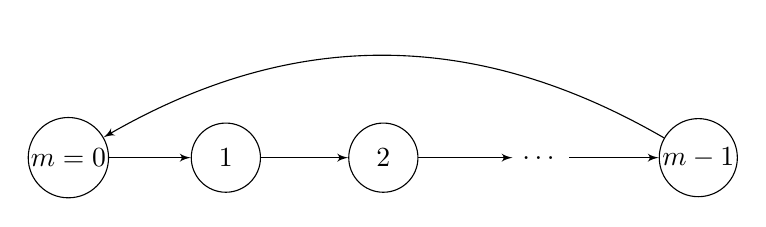
\begin{tikzpicture}
            \tikzset{vertex/.style = {shape=circle,draw,minimum size=2.5em}}
            \tikzset{edge/.style = {->,> = latex'}}
            % vertices
            \node[vertex, inner sep = 0.5pt] (0) at (0,0) {$m = 0$};
            \node[vertex] (1) at (2,0) {1};
            \node[vertex] (2) at (4,0) {2};
            \node (ellipsis) at (6,0) {\ldots};
            \node[vertex, inner sep = 0.5pt] (m-1) at (8,0) {$m-1$};
            %edges
            \draw[edge] (0) to (1);
            \draw[edge] (1) to (2);
            \draw[edge] (2) to (ellipsis);
            \draw[edge] (ellipsis) to (m-1);
            \draw[edge] (m-1) to [bend right] (0);
        \end{tikzpicture}
        \caption{Modulo $m$ number system}
    \end{figure}

        We can rigorously define the function to convert from naturals to numbers 
        modulo $m$, $n \mod m$ is the smallest number $r$ such that $n = qm + r$
        for some $q$. It's clear that $0 \leq r < m$ as if $r \geq m$, there exists $r'$ 
        such that $r = m + r'$ (proof is similar to Exercise 2.6). Substituting this, 
        we get $n = qm + m + r' = (q+1)m + r'$, so we found $r' < r$ which satisfies 
        the condition.

        This is also a well defined notation, as the set $\{ x | n = qm + x\}$ is non-
        empty. $n$ itself is in this set for $q = 0$. And any set which is non-empty 
        will have a least element, which is another way to look at the well-ordering 
        principle (Here $P(x)$ just means $x$ belongs to our set).

        Almost all operations can be defined for numbers $\mod m$. $n \mod m \ + \ k \mod m$
        is defined as $ = (n+k) \mod m$. It's also easy to show that this is commutative
        and associative by swapping around terms in the RHS. 
        Unlike the natural numbers, each number also has
        an additive inverse. This is due to the fact that if you keep adding 1 to a number,
        it will eventually loop to 0.

        How do we define an additive inverse? We must first define an additive identity,
        this is a number $a$ such that $a + n = n \ \forall n$. Clearly $a = 0$ is the 
        additive identity. The additive inverse of $n$ is a number $n'$ such that
        $n + n' = a$. The same can be defined for multiplication, and $1$ is the multiplicative identity.

        In order to talk about mutliplicative inverse, we must first define the greatest
        common divisor (gcd) of 2 numbers. For two positive numbers $a$, $b$, consider the 
        sets: \\
        $X = \{ r > 0 \mid \exists x,y \ xa = yb + r \}$ \\
        $Y = \{ r > 0 \mid \exists x,y \ xb = ya + r \}$ \\
        Both these sets aren't empty, for $x = 1$ and $y = 0$, $a, b$ belong to $X,Y$
        respectively. So each set has a well defined smallest element. The gcd of $a,b$
        is defined as the smallest element in $X \cup Y$.
        
        Another way to think about this is $X \cup Y$ is that it contains the difference
        of any multiple of $a$ with any multiple of $b$, or even can be taken as the set
        of all integer linear combinations of $a, b$ (which are positive). It's not clear that this is the 
        same as the gcd we are used to, but the properties of gcd can be proven from this 
        definition.

        What properties would we like to prove? Firstly we should check that $a \mod g = 0$
        and $b \mod g = 0$. $g$ should also be a multiple of any common divisor of $a, b$ i.e.
        if $d \mid a$ and $d \mid b$ then $d \mid g$.

        \newpage
        Let $g$ be the smallest number in $X \cup Y$. Let's take the case where $g \in X$.
        So there exists $x, y$ such that $xa = yb + g \ (1)$. Now to prove $a \mod g = 0$, let's
        assume by contradiction $a \mod g = g' \neq 0$. This can be written as $a = qg + g' \ (2)$
        from the definition of $mod$. Multiplying (1) by $q$ and adding $g'$ to both sides, we get: \\
        $qxa + g'= qyb + qg + g' = qyb + a$ (from (2)) \\
        Rearranging, $(qy)b = (qx-1)a + g'$ \\ 
        But this would mean $g' \in Y$, contradicting the fact that $g$ is the smallest element 
        in $X \cup Y$.

        The proof is identical for the other case when $g \in Y$, we get $g' \in X$
        which also leads to a contradiction. We conlcude $a \mod g = 0$. Since the 
        definition of gcd is symmetric about $a$ and $b$, we can prove using the same
        method $b \mod g$ = 0.

        Now to prove that every common divisor of $a, b$ divides $g$ too. Let $d$ be 
        such that $a \mod d = 0, b \mod d = 0$. Let $x,y$ be such that $xa = yb + g$
        \footnote{If $g \in Y$ the proof is same}. \\
        $xa \mod d = 0$ \\
        $(yb + g) \mod d = 0$ \\
        $yb \mod d + g \mod d = 0$ \\
        Since, $b \mod d = 0$, $yb \mod d = 0$, so $g \mod d = 0$ (we are done).

        \begin{exercise}
            Prove that if $a \mid bc$ and $gcd(a, b) = 1$, $a \mid c$.
        \end{exercise}
        \begin{solution}
            If $gcd(a, b) = 1$, we have integers $x,y$ such that $ax + by = 1$. Multiplying
            by $c$, $acx + bcy = c$. Since $a \mid acx$, $a \mid bcy$, $ a \mid c$. 
        \end{solution}

        \begin{exercise}
            Prove that if $p$ is prime and $p \mid ab$ then $p \mid a $ or $p \mid b$
        \end{exercise}
        \begin{solution}
            Firstly what's the definition of a prime? $p$ is prime if the only divisors
            of $p$ are 1 and $p$. The statement we want to prove is equivalent to proving
            $p \mid ab$ and $p \nmid a$ means $p \mid b$. We first show that $gcd(p,a) = 1$.
            This is fine, as if $g \mid p$, $g$ is 1 or $p$, and since $g \nmid a$, $g$ is not
            $p$, so $g$ is 1. From here the question is equivalent to the previous exercise.
        \end{solution}

        \begin{exercise}
            Are $X, Y$ in the gcd definition always the same set?
        \end{exercise}
        \begin{solution}
            Yes, they are. In fact both sets contain the gcd and all multiples of it.
            Let's prove that $X = \{ g, 2g, 3g, \dots \}$. The proof is identical for $Y$.
            Let $a' = a/g$, $b' = b/g$. Is it clear that $gcd(a',b') = 1$? Well if it wasn't
            and was equal to say $g'$, $g'$ would divide $a', b'$, and $gg'$ would divide $a, b$
            and this is a contradiction.
            
            Now if we prove we can find $x,y$ such that $xa' = yb' + 1$, we're done, as we can multiply
            both sides by $g$. We're also done if we can find $x$ such that $xa' = 1 \mod b'$.
            Here's how we show that, take the set \\
            $\{ 0, a', 2a', \dots, (b'-1)a' \}$ with $b'$ elements. We claim each element here
            is distinct mod $b'$. If 2 of them have the same remainder, say $ia'$ and $ja'$, 
            this would mean $b' \mid (i-j)a'$. But since $gcd(a',b') = 1$, $b' \mid i-j$. But 
            this is impossible as $i-j < b'$. But now that we have $b'$ distinct elements, we know
            that we can have only maximum $b'$ distinct remainders right, which means that our set
            has all the elements $\mod b'$, including the remainder 1. So we're done, there
            exists $x$ such that $xa' = 1 \mod b'$ which is the same as saying $xa' = yb' + 1$
            (for some $y$).

            Now that we've shown $g \in X$, it's clear that all multiples of $g$ are in $X$,
            as if $xa = yb + g$, $mxa = myb + mg$. All that's left to show is that the \emph{only}
            numbers in $X$ are multiples of $g$. This is also easy as if $xa = yb + r$, and 
            $g \mid xa$, $g \mid yb$, so $g \mid r$.
        \end{solution}

        \newpage
        \begin{exercise}
            Prove the fundamental theorem of arithmetic, that is every number $n$ can 
            be written uniquely as $n = p_1p_2 \dots p_k$ where the primes are written 
            in ascending order.
        \end{exercise}
        \begin{solution}
            First we prove that such a representation exists. We can do this by strong 
            induction. For $n=1$ the statement is trivial, $n=1$ is the representation.
            Now assume the statement is true for all numbers smaller than $n$. If $n$ is
            prime, $n = n$ is our representation. If $n$ is not prime, we can write 
            $n = xy$ for some $x,y > 1$. By induction assumption $x,y$ can be written as
            a product of primes, from there $n$ can be written as a product of primes.

            Now for uniqueness. Again for $n=1$ it is clear, there's no other way to write
            it. Now we'll use well ordering and proof by contradiction. Let $n$ be the 
            smallest number for which there are 2 distinct way to prime factorize it.
            Say $n = p_1p_2 \dots p_n = q_1q_2 \dots q_m$. None of $p_i, q_j$ for all $i, j$
            can be equal as if they were, we could just cancel those terms and get a smaller
            number with 2 different prime factorizations. Now WLOG assume $p_n$ is the largest
            prime in both representations. $p_n \mid q_1q_2 \dots q_m$, $p_n \nmid q_1$ as
            $p_n > q_1$, so $p_n \mid q_2 \dots q_m$. Similarly since $p_n \nmid q_2$, 
            $p_n \mid q_3 \dots q_m$. We can continue doing this and get that $p_n \mid q_m$
            which is a contradiction.
        \end{solution}

    \section{Lecture 08}

    We're going to do some questions regarding divisibility and binomial coefficients.
    To prove that $n$ is divisible by $d$, you can think of a situation where's there
    a collection of $n$ objects. If we can divide this collection into groups such that 
    each group has $d$ elements, we are done. Another way to prove is to divide the 
    collection into $d$ groups such that each group has the same number of elements.

    When we're dealing with binomial coefficients like $\binom{n}{k}$, we can think of
    this as the number of collections of $k$ objects out of $n$ objects in total.

    \begin{exercise}
        If $gcd(n,k) = 1$, prove that $k \mid \binom{n}{k}$
    \end{exercise}
    \begin{solution}
        It's possible to prove this directly. \\
        $k \binom{n}{k} = n \binom{n-1}{k-1}$. So $n$ divides $k \binom{n}{k}$ and
        since $gcd(n,k)=1$, $n$ divides $\binom{n}{k}$. But let's prove this combinatorially.

        We can think of $\binom{n}{k}$ as the number of collections with $k$ objects
        from the set $\{0, 1, \dots, n-1\}$. Suppose we have a collection $\{a_1,
        a_2, \dots a_k \}$. We claim that we can extend this to a group of $n$ collections from this 
        collection. How we do this is by adding $0, 1, 2, \dots, n-1$ to each element, 
        and taking $\mod n$. So the first collection is formed by adding $0$ to each element,
        so it's our original collection itself. For the second collection you add 1 to 
        each element, and so on.

        It's not possible that 2 groups have one common element. Suppose collection $C$ is formed
        from adding $i$ from a collection $C_1$ and $j$ from a collection $C_2$. $C_1$ and $C_2$
        have to be a part of the same group as you get one from adding $i-j$ to the other.

        How do we know these $n$ collections are distinct? Assume 2 of them are same, say the ones where
        you add $i$ and $j$ to the original collection. The difference of their sums $\mod n$ must 
        be 0, and this difference is $k(i-j)$. Since $n \mid k(i-j)$ and $gcd(n,k)=1$, $n \mid (i-j)$.
        This isn't possible as $(i-j) < n$. So now that we can bunch up all collections into groups
        of size $n$, we conclude $\binom{n}{k}$ is divisible by $n$.

        Another solution could be to divide the collections based on their sum $\mod n$. There are
        clearly $n$ groups. And for any collection in a group, you can find a corresponding collection
        in any other group by adding a suitable $i$ to each element. The proof for this is very similar. Once this is 
        shown, we basically have shown each group is of equal size. So $\binom{n}{k}$ is divisible by $n$.
    \end{solution}

    \begin{exercise}
        Is the converse of the above statement true? If $n \mid \binom{n}{k}$ can we say that
        $gcd(n,k)=1$?
    \end{exercise}
    \begin{solution}
        Nope this is false. There are actually infinitely many counterexamples.
        If we try $k = 2$ or $k = 3$ the statement is true. In fact for any prime $k$
        it doesn't work, here's a short proof.

        Since that $gcd(n,k) \neq 1$ and $k$ is prime, $gcd(n,k)=k$ i.e. $n = kq$ for 
        some $q$. $\binom{kq}{k} = \frac{(kq)(kq-1)\dots(kq-k+1)}{k!}$. If this is divisible
        by $n=kq$, $\frac{(kq-1)\dots(kq-k+1)}{k!}$ has to be an integer. But this is false, 
        none of the term in the numerator is divisible by $k$. So we'll try counterexamples 
        for $k = 4$.

        Take numbers of the form $\binom{24k+2}{4}$. This equals $\frac{(24k+2)(24k+1)(24k)(24k-1)}{(4)(3)(2)(1)} \\
        = (24k+2)[(24k+1)(k)(24k-1)]$ which is divisible by $24k+2$. But clearly $gcd(24k+2,k) = 2 \neq 1$.
    \end{solution}

    \begin{exercise}
        Prove or disprove that if $1 < k < n$ and $k \mid n$ then $n \nmid \binom{n}{k}$.
    \end{exercise}
    \begin{solution}
        This is also false. Again when $k$ is prime the statement is true, so let's first try
        $k = 4$. \\  
        $\binom{4n}{4} = (4n)\frac{(4n-1)(4n-2)(4n-3)}{(24)} = (4n)\frac{(4n-1)(2n-1)(4n-3)}{(12)}$.
        If we want to disprove the statement, the fraction must be an integer. But this isn't possible,
        as the numerator is odd.

        Let's try to construct counterexamples of the form $\binom{6n}{6}$.
        We need this to be divisible by $6n$. \\
        $\binom{6n}{6} = \frac{(6n)(6n-1)(6n-2)(6n-3)(6n-4)(6n-5)}{(720)} = 
        6n\frac{(6n-1)(3n-1)(2n-1)(3n-2)(6n-5)}{(60)}$. \\
        We just need the fraction part to simplify, let's try to find $n$ such 
        that $15 \mid (2n-1)$ and $4 \mid (3n-1)$. 
        Or equivalently, $2n = 1 \mod 15$ and $3n = 1 \mod 4$.
        For this we just to find inverses
        of $2$ and $3$ mod $15$ and $4$ respectively. That we can do, $n = 8 \mod 15$
        and $n = 3 \mod 4$. $n = 23$ (by trial and error)
        \footnote{Chinese Remainder Theorem actually guarantees a unique solution
        $\mod 60$ for this, and also gives an algorithm better than trial and error.} 
        satisfies both of these and
        adding $23$ with any multiple of $60$ will keep it the same mod $15$ and $4$.
        So $n = 60k+23$ is a set of infinite solutions. 
    \end{solution}

    \section{Lecture 09}

    We prove prime factorization in this lecture. 
    \footnote{which I already did in Exercise 7.4 but just giving what's done in class}
    A number $n>1$ is prime if it is not divisible by any number $m$ where $1 < m < n$.
    The theorem states that every number $n$ can be written uniquely as a product of prime numbers.
    We don't really care about the order of the primes in this statment, if we interchange
    primes we still consider it as the same representation. Also the primes aren't necessarily
    distinct, you could have multiple copies of the same prime. 

    So we can write $n = p_1p_2 \dots p_k$ where each $p_i$ is prime, and 
    $p_1 \leq p_2 \leq \dots \leq p_k$.

    The existence of such a representation follows from the well ordering principle.
    If there's an $n$ for which it doesn't exist, let the smallest example be $n_0$.
    There are 2 cases:
    \newpage
    \begin{enumerate}
        \item $\exists m$, $1 < m < n_0$ such that $m$ divides $n_0$
        \item There is no such $m$ i.e $n_0$ itself is prime
    \end{enumerate}        

    In our second case $n_0 = n_0$ is a valid representation. What about case 1?
    If $1 < m < n_0$, $n_0 = mq$ for some $q$ then also $1 < q < n_0$. From well
    ordering, $m$ can be written as a product of primes, $q$ can be written as 
    a product of primes $\implies n_0$ can be written as a product of primes.
    
    Now for uniqueness: suppose $n = p_1p_2 \dots p_k = q_1q_2 \dots q_m$, where \\
    $p_1 \leq p_2 \leq \dots \leq p_k$ and \\
    $q_1 \leq q_2 \leq \dots \leq q_m$ \\
    Here we're considering the smallest such $n$ for which we have 2 representations.
    We can say $p_1 \neq q_1$ as if not $n / p_1 = n / q_1$, $p_2 \dots p_k = q_2 \dots q_m$.
    So we get a smaller number wtih 2 different factorizations. WLOG $p_1 < q_1$. Since
    $p_1 \mid n$, $p_1 \mid q_i$ for some $i$. Here we're repeatedly using the fact that 
    if $a \mid bc$ and $gcd(a,b) = 1$ then $a \mid c$. We know gcd of $p_1$ with any $q_i$
    is 1 so we can keep applying this property. So we have a contradiction, we know $1 < p_1 < q_i$
    for all $i$ so it can't divide $q_i$ for any $i$.

    With our new foundation on modular arithmetic, we can now go back to defining multiplicative
    inverse. If we observe numbers modulo $p$ (usually denoted by the set $Z_p = \{0,1,\dots,p-1\})$,
    it turns out every number other than $0$ has a multiplicative inverse. The proof is similar to 
    stuff we have seen before, consider the set $a \times Z_p$ (where $a \in Z_p$, $a \neq 0$) 
    i.e. $\{0,a,2a,\dots,(p-1)a\}$.
    All these numbers will be distinct modulo $p$, as if 2 numbers were the same, their difference
    must be a multiple of $p$. That's not possible as if $p \mid (i-j)a$, $p \mid (i-j)$ or $p \mid a$,
    both of which aren't possible. This means that the set $a \times Z_p$ is just a permutation,
    and has the same elements as $Z_p$. One of these elements must be $1$ which means there
    is an $a'$ such that $aa' = 1 \mod p$. This $a'$ is the multiplicative inverse of $a$.

    Another way to convince yourself of this is that $ax = 1 \mod p$ has a solution for $x$
    $\iff gcd(a,p) = 1$.

    
    \begin{figure}[ht]
    \centering
    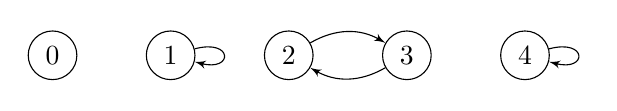
\begin{tikzpicture}
        \tikzset{vertex/.style = {shape=circle,draw,minimum size=1.5em}}
        \tikzset{edge/.style = {->,> = latex'}}
        % vertices
        \node[vertex] (0) at (0,0) {0};
        \node[vertex] (1) at (1.5,0) {1};
        \node[vertex] (2) at (3,0) {2};
        \node[vertex] (3) at (4.5,0) {3};
        \node[vertex] (4) at (6,0) {4};
        %edges
        \draw[edge] (1) to [loop right] ();
        \draw[edge] (2) to [bend left] (3);
        \draw[edge] (3) to [bend left] (2);
        \draw[edge] (4) to [loop right] ();
        
    \end{tikzpicture}

    \caption{Each number points to its inverse modulo 5}
    \end{figure}

    Another thing we can deduce from the fact that $a \times Z_p$ is the same set as 
    $Z_p$ is Fermat's Little Theorem. Ignore $0$ from both the sets and take their product.
    When we equate this, we get: $1 \times 2 \times \dots \times (p-1)
    = a \times 2a \times \dots \times (p-1)a \mod p$. Simplifying, 
    $(a^{p-1}-1)(p-1)! = 0 \mod p$ and since $gcd((p-1)!,p)=1$, $a^{p-1}=1 \mod p$. 

    Fermat's little theorem can also be used to prove EGZ theorem, which we'll see in the next
    lecture.

    \section{Lecture 10}

    We will now do another proof of EGZ theorem for the case where $n$ is prime. It's
    enough to prove this theorem for numbers belonging to $Z_p$, as we only care about 
    remainders when divided by $p$.

    Given a set $S = \{a_1, a_2, \dots, a_{2p-1}\}$, there exists a subset $A \subseteq S$,
    $|A| = p$ and $sum(A) = 0 \mod p$.

    Assume it is not true, that is for all sets the sum is not 0. Let's look at the following sum: \\
    $\sum_{A \subseteq S, |A|=p} (sum(A))^{p-1} \quad (1)$. This is just adding the sum power $p-1$ for all 
    subsets of size $p$. If none of the sums are 0, we can use FLT to show $(sum(A))^{p-1} = 1 \mod p$.
    So the weird sum we're looking at just becomes a summation of $1$, which just counts the number
    of subsets. This is clearly $\binom{2p-1}{p}$. Is this divisible by $p$? \\
    $\binom{2p-1}{p} = \frac{(2p-1)(2p-2)\dots(p)}{(p)(p-1)\dots(1)}$. The $p$'s cancel,
    and nothing else in the numerator is divisible by $p$, so no.

    We'll now show that actually the sum is $0$, by showing that each term in (1) expanded
    is $0 \mod p$. What are possible terms in the summation? For set $A = \{a_{i_1}, a_{i_2},
    \dots, a_{i_p}\}$. We multinomially expand $(a_{i_1} + \dots + a_{i_p})^{p-1}$. A general
    term of this expansion is $a_{i_1}^{k_1}a_{i_2}^{k_2} \dots a_{i_m}^{k_m}$ (call this term $t$) where 
    $1 \leq m \leq p-1$ as you can have maximum $p-1$ different $a_i$'s in a term. We also have 
    $k_1 + \dots k_m = p-1$. Note that $t$ appears multiple times in set $A$ itself, so each 
    set will have a contribution of $k \times t$. What we now prove is that the \emph{number}
    of sets $A$ for which term $t$ appears is divisible by $p$ (which makes its contribution in 
    the final sum as $0 \mod p$).
    \footnote{
    Note that if the term appears in different sets, it will appear the same number of times in 
    each set.
    }
 
    The number of sets in which the term $t$ appears is equivalent to the number of sets that 
    can be formed using the elements $a_{i_1}, a_{i_2}, \dots, a_{i_m}$. Since we have $m$
    elements already chosen and we need to choose $p$ in total, number of elements to be chosen 
    is $\binom{2p-1-m}{p-m}$. \\
    $\binom{2p-1-m}{p-m} = \frac{(2p-1-m)(2p-2-m)\dots(p)}{(p-m)(p-m-1)\dots(1)}$. Since
    there's a $p$ in the numerator, and none of the terms in the denominator are divisible
    by $p$, so the full term is divisible by $p$. 

    So we're done, we got a contradiction. We got that $(1)$ is both $0$ and not $0$ at the 
    same time.

    $2p-1$ is also a tight bound. We have proved the statement for $2p-1$ numbers, but for 
    $2p-2$ numbers we can actually get a counterexamples. Consider the set with $0$ appearing
    $p-1$ times and $1$ appearing $n-1$ times. Any $p$ numbers we choose, we'll have to choose
    2 numbers that differ. If this is the case, the sum is strictly between $0$ and $p$, which 
    means that the sum is not divisible by $p$.

    The theorem can be extended to 2 dimensions. If you have a set of $4p-3$ 2D integer coordinates,
    You can find $p$ of them with their centroid (basically mean of both coordinates) as an
    integer. This theorem was proven and again there's a counterexample with $4p-4$ points. Take 
    the set: \\
    $\{ \binom{0}{0}, \dots, \binom{0}{0}, \binom{0}{1}, \dots, \binom{0}{1}, 
    \binom{1}{0}, \dots, \binom{1}{0}, \binom{1}{1}, \dots , \binom{1}{1}\}$ where each point
    appears $p-1$ times. You will have to choose 2 unequal points, and in whichever coordinate they
    are unequal, that coordinate's sum will be strictly between $0$ and $p$.

    Another theorem we can prove for primes is \textbf{Wilson's Theorem: }a number $n$
    is prime $\iff$ $(n-1)!+1 = 0 \mod n$. 

    The proof of Wilson's Theorem follows from the fact that every number in $Z_p$ (except 0)
    has a unique inverse. So while multiplying all of them, we can just pair each element with 
    its inverse and it will become multiplication of a bunch of $1$'s. But we have to be a bit 
    careful, as what if a number is the inverse of itself? If $a^2 = 1 \mod p$, $(a+1)(a-1)
    = 0 \mod p$. $p \mid (a-1)$ or $p \mid (a+1)$ which means $a = 1$ or $a = p-1$. So ignoring
    these 2 numbers, if we multiply the rest, the product is $1 \mod p$. Including $1$ and $p-1$ now,
    the product is $(p-1) \mod p$, so $(p-1)! + 1 = (p-1) + 1 = 0 \mod p$. 
    
    \newpage
    The converse isn't too hard to prove. 
    One number in $(p-1)!$ will be a divisor of $p$ (say $k > 1$), which will make $(p-1)!$
    also divisible by $k$. Even while taking this modulo $p$, the remainder will be divisible by $k$ as
    if $(p-1)! = qp + r$, $k \mid (p-1)!$, $k \mid p$, so $k \mid r$. From here we can say $r \neq p-1$
    as if $k \mid r = p-1$ and $k \mid p$, $k \mid p - (p-1) = 1$.

    Wilson's theorem is true both ways and can be used as a test for primes, although not efficient.
    The same can't be said for FLT, it is possible when there's a composite $n$, $gcd(a,n)=1$,
    and $a^{n-1} = 1 \mod n$. In fact there are numbers called Carmichael numbers (pseudo primes).
    These are the strongest counterexamples, they are composite $n$ such that for \emph{all}
    $a$ such that $gcd(a,n)=1$, $a^{n-1}=1 \mod n$. The first 3 Carmichael numbers are 561, 1105, and 
    1729.

    There is a way to improve FLT to test more accurately for primes, called the Miller
    Rabin primality test. It's based on FLT as well as the fact that if  $x^2 = 1 \mod n$,
    $x = 1 \mod n $ or $x = n-1 \mod n$. To test if $n$ is prime, we pick a random number
    $1 < a < n$. If $a^{n-1} \neq 1 \mod n$, we confirm $n$ is composite. But if it's equal,
    we're still not guaranteed that $n$ is prime. What we do is we divide the exponent by $2$
    whenever possible, and check if it's still $\pm 1 \mod n$. So we check $a^{\frac{n-1}{2}} \mod n$.
    If it's not $\pm 1 \mod n$, $n$ is composite. If it's $1 \mod n$ and the exponent is still
    even, we can continue this process and check for $a^{\frac{n-1}{4}} \mod n$. If it's 
    $-1 \mod n$, or the exponent becomes odd, we stop, as we can't apply the property anymore.

    Even this test doesn't guarantee if $n$ is prime or composite, but it's better than just 
    plain FLT, as we are checking more. If we do this process for more and more $a$'s, our guarantee
    that $n$ is prime becomes more and more certain. If we ever get that $n$ is composite 
    from the test, we are 100\% sure that it is composite. But if can't disprove $n$ is prime, 
    we are never completely sure that $n$ is prime.

    \section{Lecture 11}

    This lecture is basically discussion of 2 questions in the previous year's quiz.

    \begin{exercise}
        Find natural numbers $n$, $0 \leq n < 1000$ such that $n^2$ has the same ending 3 digits 
        as $n$. Let's generalize this question. What are the number of solutions $0 \leq n < b^d$ 
        such that $n^2$ has the same $d$ ending digits as $n$? It's given that $b$ has a prime 
        factorization $p_1^{k_1}p_2^{k_2} \dots p_m^{k_m}$
    \end{exercise}

    \begin{solution}
        Here's a proof for the general case, just substitute $b = 10$ and $d = 3$ for 
        the first part. When we say the $d$ ending digits are same, we just mean that 
        $b^d \mid (n^2-n)$ or $b^d \mid n(n-1)$. Since $b^d = p_1^{dk_1}p_2^{dk_2} \dots p_m^{dk_m}$,
        it is enough to verify that $p_i^{dk_i} \mid n(n-1)$ for all $i$.
        \footnote{This follows from the fact that if $gcd(d_1,d_2) = 1$, $d_1 \mid n$ and 
        $d_2 \mid n$ $\iff$ $d_1d_2 \mid n$. This can be proved using Exercise 7.1}

        Now since $gcd(n,n-1)=1$, $p_i^{dk_i} \mid n(n-1)$ is equivalent to $ p_i^{dk_i} \mid n$
        or $p_i^{dk_i} \mid (n-1)$. This is like an exclusive or also, we can't have both at the 
        same time. So for every $i$ we have a choice, we could make the term divide $n$ or 
        divide $n-1$. So there are $2^m$ total choices.

        Now for each choice, do we always have a solution, and how many solutions do we have?
        For the extreme cases, when everything has to divide $n$, $n=0$ is the solution. When
        everything has to divide $n-1$, $n=1$ is the solution, but we can't keep checking every
        case manually. Let's say we choose some $d_1$ of these terms to divide $n$ and the rest
        $d_2$ terms to divide $n-1$. Denote the product of the $d_1$ terms to be $t_1$, product
        of the $d_2$ terms to be $t_2$. We have $t_1t_2 = b^d$.

        Since $t_1 \mid n$, we can write $n = qt_1$. To keep $n$ in our range, $0 \leq q < t_2$.
        We need $t_2 \mid n-1 = qt_1-1$ which is basically $qt_1 = 1 \mod t_2$. This is the same
        as saying $q$ is the inverse of $t_1 \mod t_2$. And since $gcd(t_1, t_2) = 1$, $q$ exists
        and is unique. So for each choice we have exactly $1$ solution, so our final answer is $2^m$.
        
    \end{solution}

    \begin{exercise}
        If $\alpha, \beta$ are irrational and $1/\alpha + 1/\beta = 1$, show that for every integer 
        $n$, there exists $k$ such that $n = \floor{k\alpha}$ or $n = \floor{k\beta}$.
        If $\alpha, \beta$ are rational a general solution can be written as $\alpha = \frac{p}{q}$
        and $\beta = \frac{p}{p-q}$ ($gcd(p,q)=1$). For which $n$ (if any) is the statment false? 
    \end{exercise}

    \begin{solution}
        One of the fractions $1/\alpha$, $1/\beta$ must be greater than half. WLOG take it
        to be the first one i.e. $\alpha < 2$. Because it's smaller than $2$, if we think about
        the set $\{\floor{\alpha}, \floor{2\alpha}, \floor{3\alpha}, \dots\}$, it can only skip
        1 number in a row. If it skips a particular $n$, we try to show that there is a $k$ 
        such that $\floor{k\beta} = n$.

        When it skips a particular $n$, say $\floor{k\alpha} = n-1$ and 
        $\floor{(k+1)\alpha} = n+1$
        So the first equation can be written like $n-1 < k\alpha < n$. Note that there's no equality
        as $\alpha$ is irrational. Let's try to manipulate this to be in terms of $\beta$. \\
        $\frac{k}{n-1} > \frac{1}{\alpha} > \frac{k}{n}$ \\
        $\frac{k}{n-1} > 1 - \frac{1}{\beta} > \frac{k}{n}$ \\
        Simplifying, we get $(n-k)\beta > n$ and $(n-k-1)\beta < n-1$. \\
        We can do this for the other inequality too (or just sub $n=n+2$ and $k=k+1$), we get: \\
        $(n-k)\beta < n+1$ and $(n-k+1)\beta < n+2$. \\
        Now from these inequalities, we get $\floor{(n-k)\beta} = n$ so we have found $k' = n-k$
        for which $\floor{k'\beta} = n$.

        In the case of rationals, the only change in our proof is equality in a few inequalities.
        The changes are $n-1 \leq k\alpha < n$ and $ n+1 \leq \floor{(k+1)\alpha} < n+2$.
        This changes the inequality in the last step to $(n-k)\beta \leq n+1$. So our proof
        fails for rationals whenever equality occurs. Tracing this back, it is when $(k+1)\alpha = n+1$.
        i.e. $n = (k+1)\frac{p}{q} - 1$. Since $n$ is natural and $gcd(p,q)=1$, $\frac{k+1}{q}$
        must be an integer, say $k'$. So $n = k' - 1$. Our proof for rationals fails 
        whenever $n = -1 \mod p$.

    \end{solution}


\end{document}